\documentclass[12pt]{article}

\usepackage[utf8]{inputenc}
\usepackage[T1]{fontenc}
\usepackage{amsmath}
\usepackage[margin=1.0in]{geometry}


\title{Term structure model in \texttt{StocVal}}
\author{Nathan Esau}
\date{\today}

\usepackage{Sweave}
\begin{document}
\Sconcordance{concordance:pricing_kernel_demo.tex:pricing_kernel_demo.Rnw:%
1 12 1 1 0 53 1 1 2 1 0 1 2 1 0 1 3 2 0 1 3 2 0 1 2 1 0 1 3 2 0 1 1 102 %
0 2 1 3 0 1 2 2 1 1 2 10 0 1 1 10 0 1 2 3 1 1 2 1 0 1 3 2 0 2 1 9 0 1 1 %
10 0 1 2 3 1 1 2 1 0 8 1 1 4 2 0 1 4 2 0 1 2 1 15 17 0 1 2 3 1 1 3 2 0 %
1 1 4 0 1 2 1 3 2 0 1 1 4 0 1 2 1 3 2 0 1 1 4 0 1 2 1 3 2 0 1 1 4 0 1 2 %
1 1}


\maketitle

\section{Pricing Kernel}

In the master thesis of C.C. Slagmolen, Economic Scenarios for an Asset and Liability Management
Study of a Pension Fund (2010), a pricing kernel approach to generating a term structure of interest rates
is presented.

\subsection{Formulas}

\medskip
The pricing kernel is related to the state variable as 

\begin{align}
-m_{t+1} &= \delta_0 + \delta_1 z_t + 0.5 \lambda_t ' \lambda_t + \lambda_t' \epsilon_{t+1} \\
\lambda_t &= \lambda_0 + \lambda_1 z_t
\end{align}

Later on they show that in fact

\begin{align}
B_{n+1}' &= -\delta_1 + B_n' \Phi - B_{n}' \lambda_1 \\
A_{n+1} &= -\delta_0 + A_n + B_n'v - B_n'\Sigma\lambda_0 + 0.5 B_n'\Sigma\Sigma'B_n \\
p_{t}^{(n)} &= A_n + B_n' z_t \\
y_{t}^{(n)} &= -\frac{A_n}{n} - \frac{B_n'}{n} z_t 
\end{align}

where $y_{t}^{(n)}$ is the $(n)$ year continuous spot rate at time $t$ and $p_{t}^(n)$ 
is the log bond price for an $n$-year nominal bond at time $t$.

\medskip
Essentially, all we need to estimate is $\Phi$, the VAR coefficients, $\Sigma$, the VAR
covariance matrix, and we need to estimate $\Sigma \lambda_0$ and $\Sigma \lambda_1$ 
for the pricing kernel, conditional on $\Sigma$ and $\Phi$.

\medskip
Calculating $\Sigma \lambda_0$ and $\Sigma \lambda_1$ is a bit tricky. This is done
by minimizing the sum of squared errors between the fitted yields and the historical
yields for 2, 3, 5, and 10 year bonds over the historical period (in this case over 20 years).
In the end we need to estimate 11 unknown parameters. We can minimize the sum of squares
using the \texttt{R optim} function.

\subsection{Historical Fit}

\medskip
Below, the code to generate the model is shown and the fit with the historical term structure
yields is plotted. For simplicity, a 4 component VAR containing the 1-month treasury bill yield,
the inflation rate, the 10-year treasury bond yield and the stock index (described in more 
detail in vignettes \texttt{var\_canada\_summary.pdf} and \texttt{data\_used.pdf}) was calibrated
to historical data from 1995 to 2015.

\begin{Schunk}
\begin{Sinput}
> library(StocVal)
> marketData <- 
+   readRDS("~/Dropbox/Research/StocVal/data/Canada/varinput_canada.Rda")
> varData <- data.frame(onemonth=marketData$onemonth,
+   inflation=marketData$inflation, tenyear=marketData$tenyear,
+   stock=marketData$stock)
> histYields <- data.frame(twoyear=marketData$twoyear, 
+   threeyear=marketData$threeyear, fiveyear=marketData$fiveyear, 
+   tenyear=marketData$tenyear)
> mu <- matrix(c(mean(varData$onemonth), mean(varData$inflation),
+   mean(varData$tenyear), mean(varData$stock)), 4, 1)
> varData <- data.frame(onemonth=varData$onemonth - mu[1], 
+   inflation=varData$inflation - mu[2], tenyear=varData$tenyear-mu[3],
+   stock=varData$stock - mu[4])
> var_ols.out <- var_ols(varData)
\end{Sinput}
\begin{Soutput}
VAR Estimation Results:
========================= 
Endogenous variables: onemonth, inflation, tenyear, stock 
Deterministic variables: none 
Sample size: 244 
Log Likelihood: 4999.122 
Roots of the characteristic polynomial:
0.9858 0.9662 0.8646 0.1645
Call:
VAR(y = varData, p = 1, type = "none")


Estimation results for equation onemonth: 
========================================= 
onemonth = onemonth.l1 + inflation.l1 + tenyear.l1 + stock.l1 

               Estimate Std. Error t value Pr(>|t|)    
onemonth.l1   0.9864638  0.0136533  72.251   <2e-16 ***
inflation.l1 -0.0011551  0.0013884  -0.832    0.406    
tenyear.l1    0.0027994  0.0143299   0.195    0.845    
stock.l1      0.0001222  0.0002526   0.484    0.629    
---
Signif. codes:  0 ‘***’ 0.001 ‘**’ 0.01 ‘*’ 0.05 ‘.’ 0.1 ‘ ’ 1


Residual standard error: 0.0001704 on 240 degrees of freedom
Multiple R-Squared: 0.9871,	Adjusted R-squared: 0.9869 
F-statistic:  4596 on 4 and 240 DF,  p-value: < 2.2e-16 


Estimation results for equation inflation: 
========================================== 
inflation = onemonth.l1 + inflation.l1 + tenyear.l1 + stock.l1 

              Estimate Std. Error t value Pr(>|t|)    
onemonth.l1   0.378592   0.329299   1.150    0.251    
inflation.l1  0.867740   0.033487  25.913   <2e-16 ***
tenyear.l1   -0.120277   0.345617  -0.348    0.728    
stock.l1      0.005057   0.006093   0.830    0.407    
---
Signif. codes:  0 ‘***’ 0.001 ‘**’ 0.01 ‘*’ 0.05 ‘.’ 0.1 ‘ ’ 1


Residual standard error: 0.004109 on 240 degrees of freedom
Multiple R-Squared: 0.774,	Adjusted R-squared: 0.7702 
F-statistic: 205.4 on 4 and 240 DF,  p-value: < 2.2e-16 


Estimation results for equation tenyear: 
======================================== 
tenyear = onemonth.l1 + inflation.l1 + tenyear.l1 + stock.l1 

               Estimate Std. Error t value Pr(>|t|)    
onemonth.l1   0.0183055  0.0122124   1.499    0.135    
inflation.l1 -0.0020458  0.0012419  -1.647    0.101    
tenyear.l1    0.9684399  0.0128176  75.556   <2e-16 ***
stock.l1     -0.0001873  0.0002260  -0.829    0.408    
---
Signif. codes:  0 ‘***’ 0.001 ‘**’ 0.01 ‘*’ 0.05 ‘.’ 0.1 ‘ ’ 1


Residual standard error: 0.0001524 on 240 degrees of freedom
Multiple R-Squared: 0.9877,	Adjusted R-squared: 0.9875 
F-statistic:  4824 on 4 and 240 DF,  p-value: < 2.2e-16 


Estimation results for equation stock: 
====================================== 
stock = onemonth.l1 + inflation.l1 + tenyear.l1 + stock.l1 

             Estimate Std. Error t value Pr(>|t|)  
onemonth.l1  -0.67979    3.46714  -0.196   0.8447  
inflation.l1 -0.73870    0.35258  -2.095   0.0372 *
tenyear.l1    2.93977    3.63895   0.808   0.4200  
stock.l1      0.15850    0.06415   2.471   0.0142 *
---
Signif. codes:  0 ‘***’ 0.001 ‘**’ 0.01 ‘*’ 0.05 ‘.’ 0.1 ‘ ’ 1


Residual standard error: 0.04327 on 240 degrees of freedom
Multiple R-Squared: 0.05821,	Adjusted R-squared: 0.04252 
F-statistic: 3.709 on 4 and 240 DF,  p-value: 0.005979 



Covariance matrix of residuals:
           onemonth  inflation   tenyear      stock
onemonth  2.859e-08  8.212e-08 3.674e-09  2.445e-07
inflation 8.212e-08  1.688e-05 4.320e-08 -1.798e-05
tenyear   3.674e-09  4.320e-08 2.259e-08  3.651e-07
stock     2.445e-07 -1.798e-05 3.651e-07  1.872e-03

Correlation matrix of residuals:
          onemonth inflation tenyear    stock
onemonth   1.00000   0.11819 0.14458  0.03342
inflation  0.11819   1.00000 0.06995 -0.10115
tenyear    0.14458   0.06995 1.00000  0.05615
stock      0.03342  -0.10115 0.05615  1.00000
\end{Soutput}
\begin{Sinput}
> Phi <- var_ols.out$Phi
> Sigma <- var_ols.out$Sigma
\end{Sinput}
\end{Schunk}

The VAR components estimated under OLS, $\Phi$ and $\Sigma$ are shown below.

\begin{Schunk}
\begin{Sinput}
> print(Phi)
\end{Sinput}
\begin{Soutput}
            [,1]         [,2]         [,3]          [,4]
[1,]  0.98646376 -0.001155122  0.002799417  0.0001222493
[2,]  0.37859226  0.867739719 -0.120277410  0.0050566611
[3,]  0.01830546 -0.002045783  0.968439896 -0.0001873244
[4,] -0.67978830 -0.738696384  2.939772604  0.1584992165
\end{Soutput}
\begin{Sinput}
> print(Sigma)
\end{Sinput}
\begin{Soutput}
              onemonth     inflation      tenyear         stock
onemonth  2.859137e-08  8.211634e-08 3.674473e-09  2.444751e-07
inflation 8.211634e-08  1.688483e-05 4.320068e-08 -1.798383e-05
tenyear   3.674473e-09  4.320068e-08 2.258991e-08  3.651185e-07
stock     2.444751e-07 -1.798383e-05 3.651185e-07  1.872010e-03
\end{Soutput}
\end{Schunk}

Next, we calculate $\Sigma\lambda_0$ and $\Sigma\lambda_1$. Note that this
requires minimizing a function of 11 variables, which can take several minutes.

\begin{Schunk}
\begin{Sinput}
> N <- c(2,3,5,10)
> varData <- data.frame(onemonth=marketData$onemonth,
+   inflation=marketData$inflation, tenyear=marketData$tenyear,
+   stock=marketData$stock)
> calibrate_VAR.out <- calibrate_VAR(varData, histYields, Phi, Sigma, N)
> print(calibrate_VAR.out$SigmaL0)
\end{Sinput}
\begin{Soutput}
              [,1]
[1,] -0.0008554283
[2,]  0.0000000000
[3,]  0.0043091028
[4,]  0.1093473720
\end{Soutput}
\begin{Sinput}
> print(calibrate_VAR.out$SigmaL1)
\end{Sinput}
\begin{Soutput}
            [,1]         [,2]        [,3]         [,4]
[1,]  0.04023035  0.007023689 -0.01917770 -0.001333910
[2,]  0.00000000  0.000000000  0.00000000  0.000000000
[3,]  0.07901779 -0.067519345 -0.03387606  0.002708078
[4,] -0.67978830 -0.738696384  2.93977260  0.158499216
\end{Soutput}
\end{Schunk}

Next, we calculate the fitted historical yields, having solved for $\Sigma\lambda_0$
and $\Sigma\lambda_1$. 

\begin{Schunk}
\begin{Sinput}
> SigmaL0 <- calibrate_VAR.out$SigmaL0
> SigmaL1 <- calibrate_VAR.out$SigmaL1 
> ncomponents <- length(Phi[,1]) # number of VAR components
> delta1 <- c(1,0,0,0) # 1 corresponds to 1 month short rate
> nrows <- length(varData[,1]) # varData and histYields are same length
> An <- c(0)
> Bnt <- matrix(rep(0,ncomponents),1,ncomponents)
> total <- 0
> nsum_index <- 1
> A <- function(An, Bnt, SigmaL0, Sigma) { # An
+   An - Bnt %*% SigmaL0 + 0.5 * Bnt %*% Sigma %*% t(Sigma) %*% t(Bnt)
+ }
> B <- function(Bnt, Phi, delta1, SigmaL1) { # Bnt
+   -delta1 + Bnt %*% Phi - Bnt %*% SigmaL1 
+ }
> fittedYields <- vector("list", ncomponents)
> for(n in 1:(max(N))) {
+   An <- A(An, Bnt, SigmaL0, Sigma)
+   Bnt <- B(Bnt, Phi, delta1, SigmaL1)
+   if(is.element(n,N)) { # loop over t
+     fittedYields[[nsum_index]] <- numeric(nrows)
+     yields <- histYields[,nsum_index]
+     for(t in 1:nrows) {
+       zt <- matrix(as.numeric(varData[t,]), ncomponents, 1)
+       pt <- An + Bnt %*% zt
+       yt_fit <- -pt/n # fitted yield
+       fittedYields[[nsum_index]][t] <- yt_fit
+     }
+     nsum_index <- nsum_index + 1 # next column of histYields
+   }
+ }
\end{Sinput}
\end{Schunk}

The plots are shown below comparing the historical yields (in blue)
with the fitted yields (in red) for 2, 3, 5 and 10 year bonds.

\begin{Schunk}
\begin{Sinput}
> plot(ts(histYields[[1]], start=1995, end=2015, freq=12), ylab="2-year", 
+   type='l', col='blue', main="2-year historical yield fit")
> lines(ts(fittedYields[[1]], start=1995, end=2015, freq=12), type='l', col='red')
\end{Sinput}
\end{Schunk}
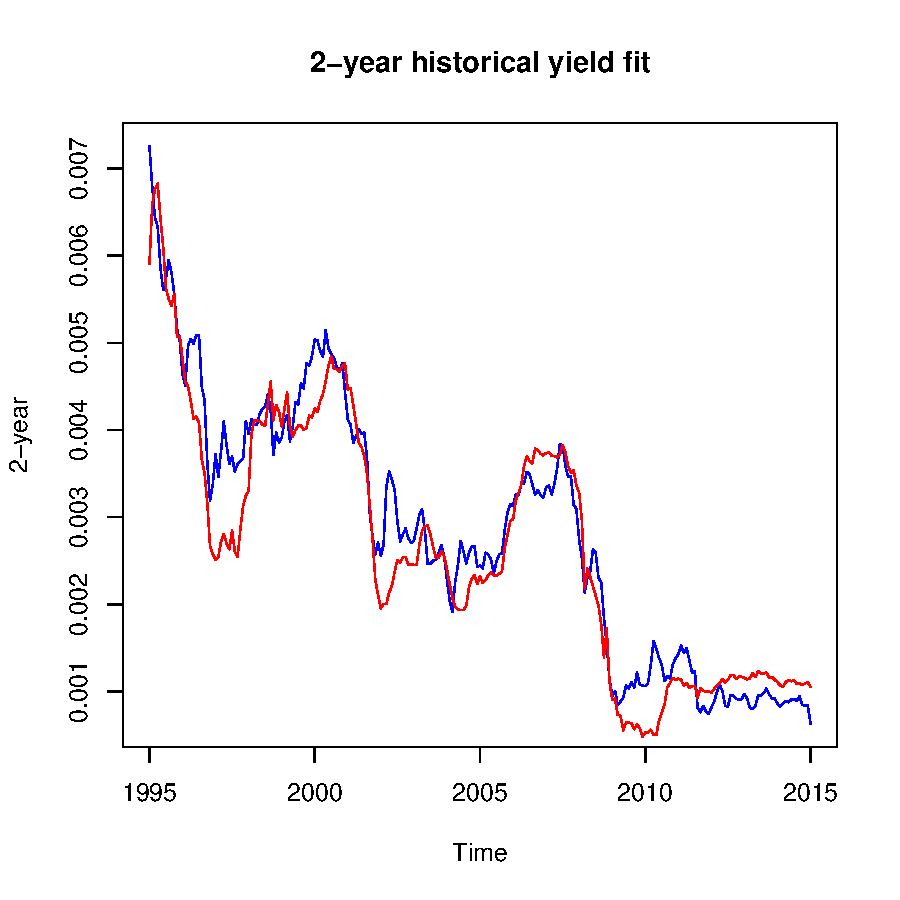
\includegraphics{pricing_kernel_demo-005}

\begin{Schunk}
\begin{Sinput}
> plot(ts(histYields[[2]], start=1995, end=2015, freq=12), ylab="3-year", 
+   type='l', col='blue', main="3-year historical yield fit")
> lines(ts(fittedYields[[2]], start=1995, end=2015, freq=12), type='l', col='red')
\end{Sinput}
\end{Schunk}
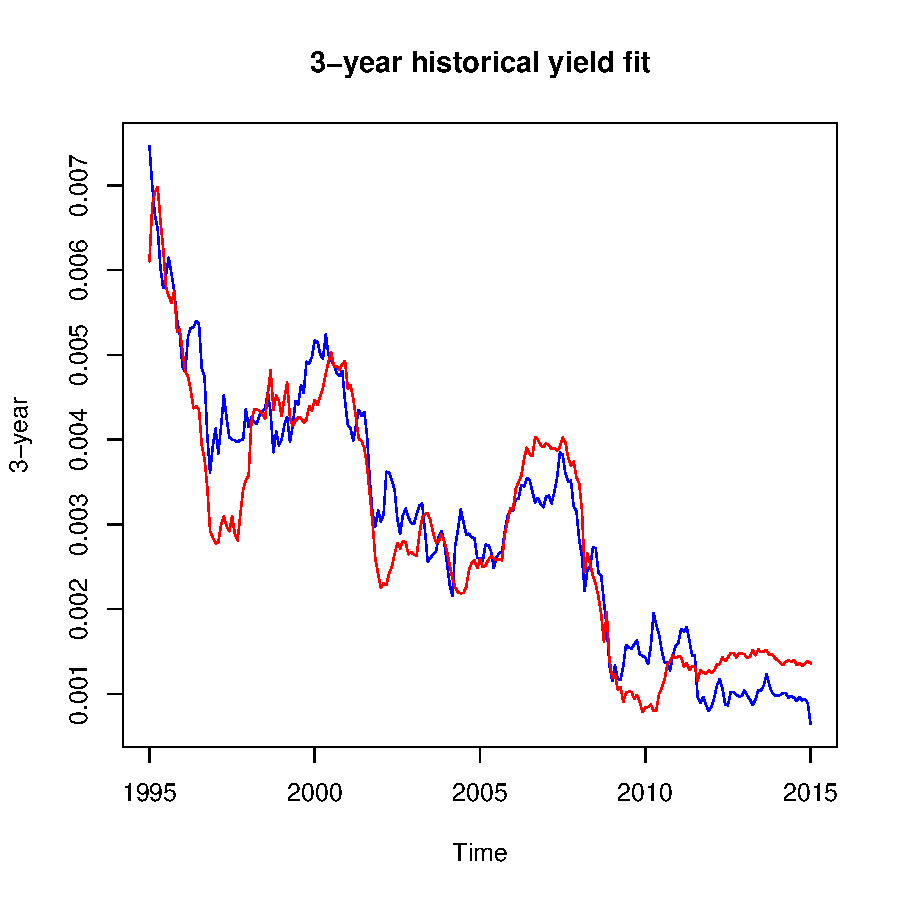
\includegraphics{pricing_kernel_demo-006}

\begin{Schunk}
\begin{Sinput}
> plot(ts(histYields[[3]], start=1995, end=2015, freq=12), ylab="5-year", 
+   type='l', col='blue', main="5-year historical yield fit")
> lines(ts(fittedYields[[3]], start=1995, end=2015, freq=12), type='l', col='red')
\end{Sinput}
\end{Schunk}
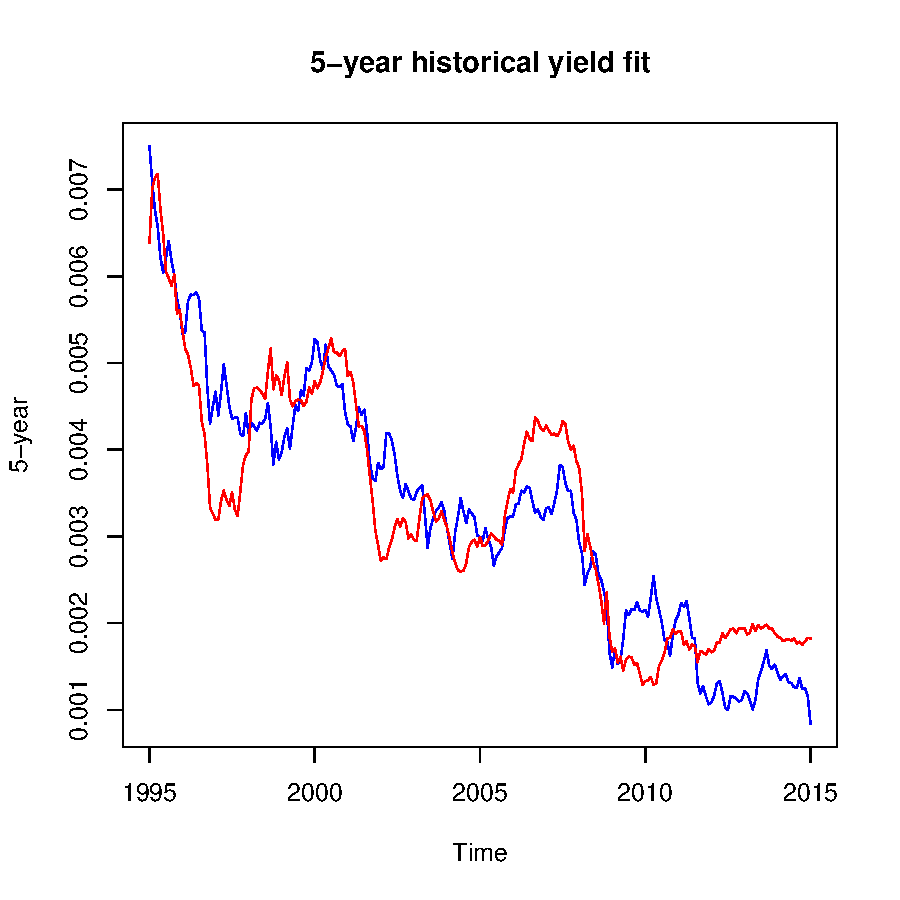
\includegraphics{pricing_kernel_demo-007}

\begin{Schunk}
\begin{Sinput}
> plot(ts(histYields[[4]], start=1995, end=2015, freq=12), ylab="10-year", 
+   type='l', col='blue', main="10-year historical yield fit")
> lines(ts(fittedYields[[4]], start=1995, end=2015, freq=12), type='l', col='red')
\end{Sinput}
\end{Schunk}
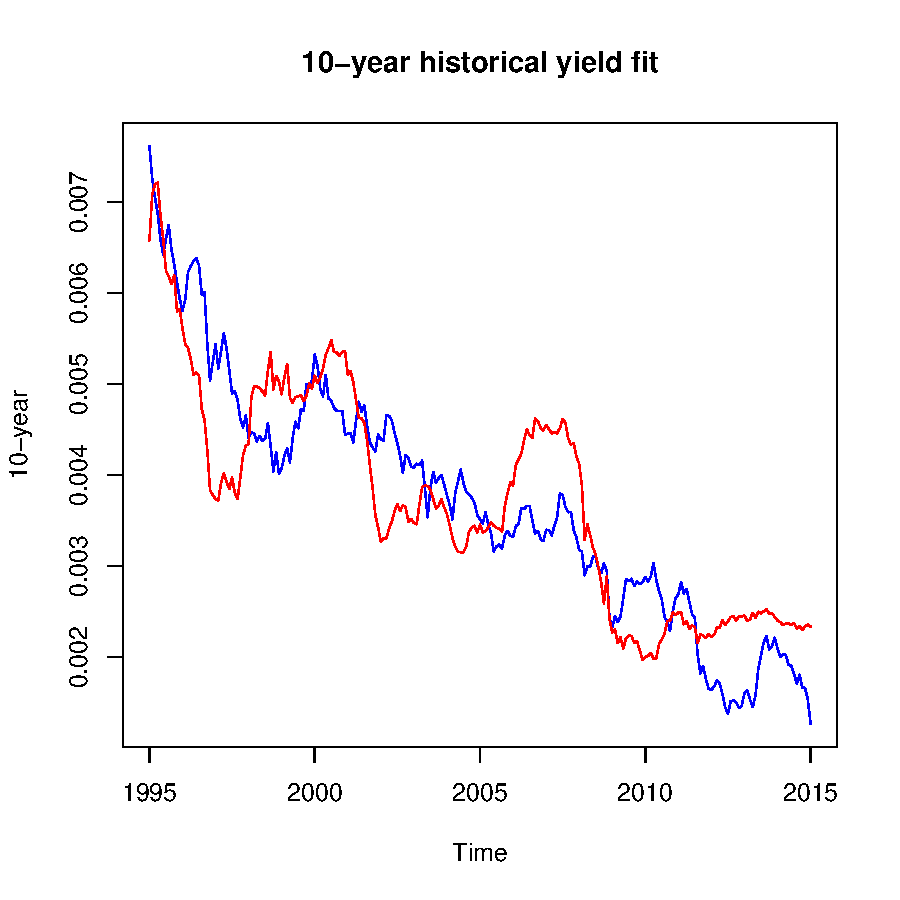
\includegraphics{pricing_kernel_demo-008}

\end{document}
